\documentclass[10pt,a4paper]{article}
\usepackage[T1]{fontenc}
\usepackage[utf8]{inputenc}
\usepackage{lmodern}
\usepackage[textwidth=483pt,top=43pt,bottom=46pt]{geometry}
\usepackage{amsmath,amssymb,graphicx,booktabs,longtable}
\usepackage[colorlinks=true,linkcolor=blue,urlcolor=blue]{hyperref}
\hypersetup{pdftitle={AI Data Center Power and Compute Co Scheduling},pdfauthor={HackSHSID 2026 project}}
\setlength{\parindent}{0pt}
\setlength{\parskip}{6pt}
\setlength{\footskip}{20pt}
\setlength{\emergencystretch}{2em}
\renewcommand{\baselinestretch}{1.08}
\pagestyle{plain}
\begin{document}
{\raggedright\LARGE\bfseries AI Data Center\\ Power and Compute Co-Scheduling\par}\vspace{1em}

{\small HackSHSID 2026 Track 2 | Public-data study | 2020-06-01 energy day\par}

\subsection*{Purpose and result}

Flexible computing and batteries both move electricity demand across time. We coordinate non-preemptive GPU job starts and two storage layers to reduce operating cost while preserving admitted work and an explicit carbon policy.

All 26 jobs finish before their assumed deadlines. Joint green reduces modeled cost by 10.97\% and peak import by 30.62\%, while meeting a chosen 3\% carbon-accounting reduction. Both batteries restore initial energy.

\begin{center}\begingroup\setlength{\tabcolsep}{4pt}
\renewcommand{\arraystretch}{1.2}
\fontsize{8.5}{11.90}\selectfont
\begin{tabular}{@{}p{236.88pt}p{115.06pt}p{115.06pt}@{}}
\toprule
\textbf{Metric} & \textbf{FIFO} & \textbf{Joint green} \\
\midrule
Cost proxy / CNY per day & 230.85 & 205.54 \\
Carbon accounting / kg CO2 & 97.67 & 94.74 \\
Peak grid import / kW & 42.55 & 29.52 \\
Modeled GPU-hours & 762.00 & 762.00 \\
\bottomrule\end{tabular}\endgroup\end{center}

\begin{center}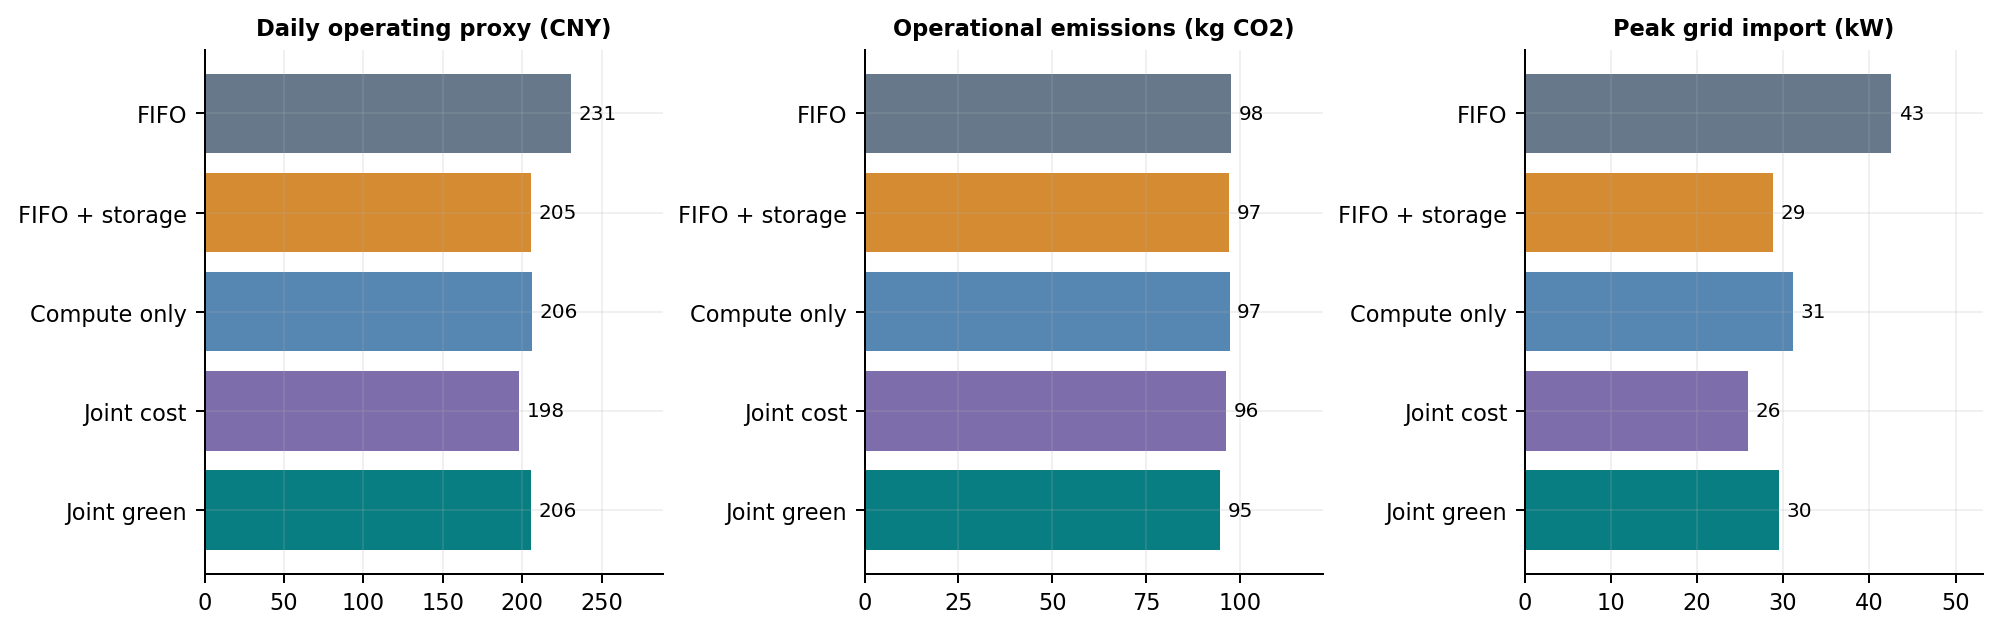
\includegraphics[width=\linewidth,height=180pt,keepaspectratio]{figures/comparison.png}\end{center}
{\small Figure 1. Same admitted workload; all five saved policies independently audited.\par}

The benchmark combines observed Helios GPU jobs, OPSD British electricity/solar records and UK carbon estimates. It is a counterfactual composite, not a measured British facility: deadlines, power, assets, currency conversion, national-solar scaling and workload relocation remain assumptions.

{\small SciPy/HiGHS solves a start-indexed mixed-integer linear program. The green objective gap is 0.000055\%. Other public dates include unattainable targets; constructed stresses include negative cost savings. Neither failures nor work are discarded.\par}

\clearpage
\section*{2  Data and study assumptions}
\begin{center}\begingroup\setlength{\tabcolsep}{4pt}
\renewcommand{\arraystretch}{1.2}
\fontsize{8.3}{11.62}\selectfont
\begin{tabular}{@{}p{98.34pt}p{376.66pt}@{}}
\toprule
\textbf{Input} & \textbf{Source and transformation} \\
\midrule
GPU jobs & Helios Saturn / vcOIr: completed GPU jobs, 1,800-10,800 s, submitted before 18:00; first at most 32 by submission then source ID \\
Capacity/background & 192 published VC GPUs; fixed background is each slot's maximum concurrency from same-VC completed GPU jobs shorter than 1,800 s \\
Electricity & OPSD GB\_GBN\_price\_day\_ahead, GBP/MWh x assumed 9 CNY/GBP / 1,000; negative prices retained \\
Solar & OPSD actual national solar MW x assumed 0.004 kW/MW; missing capacity factors are not filled \\
Carbon & UK national API actual field, estimated average g CO2/kWh / 1,000 \\
\bottomrule\end{tabular}\endgroup\end{center}

The 26 source jobs retain IDs, CSV rows, GPU counts, submit/start/end times and execution seconds. Upward 15-minute rounding gives 762.00 modeled GPU-hours from 693.86 observed GPU-hours (9.82\% padding). Deadlines allow up to four hours waiting after rounded duration, capped at day end. No dependency graph or inference label is invented.

Energy records align to UTC interval starts. Helios timestamps have no documented timezone; within-day offsets are rebased onto the modeled British day. Hourly/half-hourly observations are held constant, without interpolated noise. The completed-job subset is not a representative sample of all Helios work.

\begin{center}\begingroup\setlength{\tabcolsep}{4pt}
\renewcommand{\arraystretch}{1.2}
\fontsize{8.5}{11.90}\selectfont
\begin{tabular}{@{}p{265.53pt}p{209.47pt}@{}}
\toprule
\textbf{Assumption} & \textbf{Configured value} \\
\midrule
Base / active or reserved GPU / PUE & 20 kW / 0.25 kW per GPU / 1.20 \\
Facility / grid / successive ramp & 150 kW / 120 kW / 50 kW per step \\
Renewable cost / daily peak proxy & 0.06 CNY/kWh / 2 CNY per kW-day \\
LFP / sodium-ion capacity & 40 kWh / 6 kWh \\
\bottomrule\end{tabular}\endgroup\end{center}

{\small Helios is commit/archive-hash pinned. OPSD's database was recovered through a pinned archive mirror and exactly matches the publisher's SHA-256; the mirror is a transport route. Source excerpts, metadata, terms and hashes ship in data/raw/. Missing/corrupted required observations fail explicitly.\par}

\begin{center}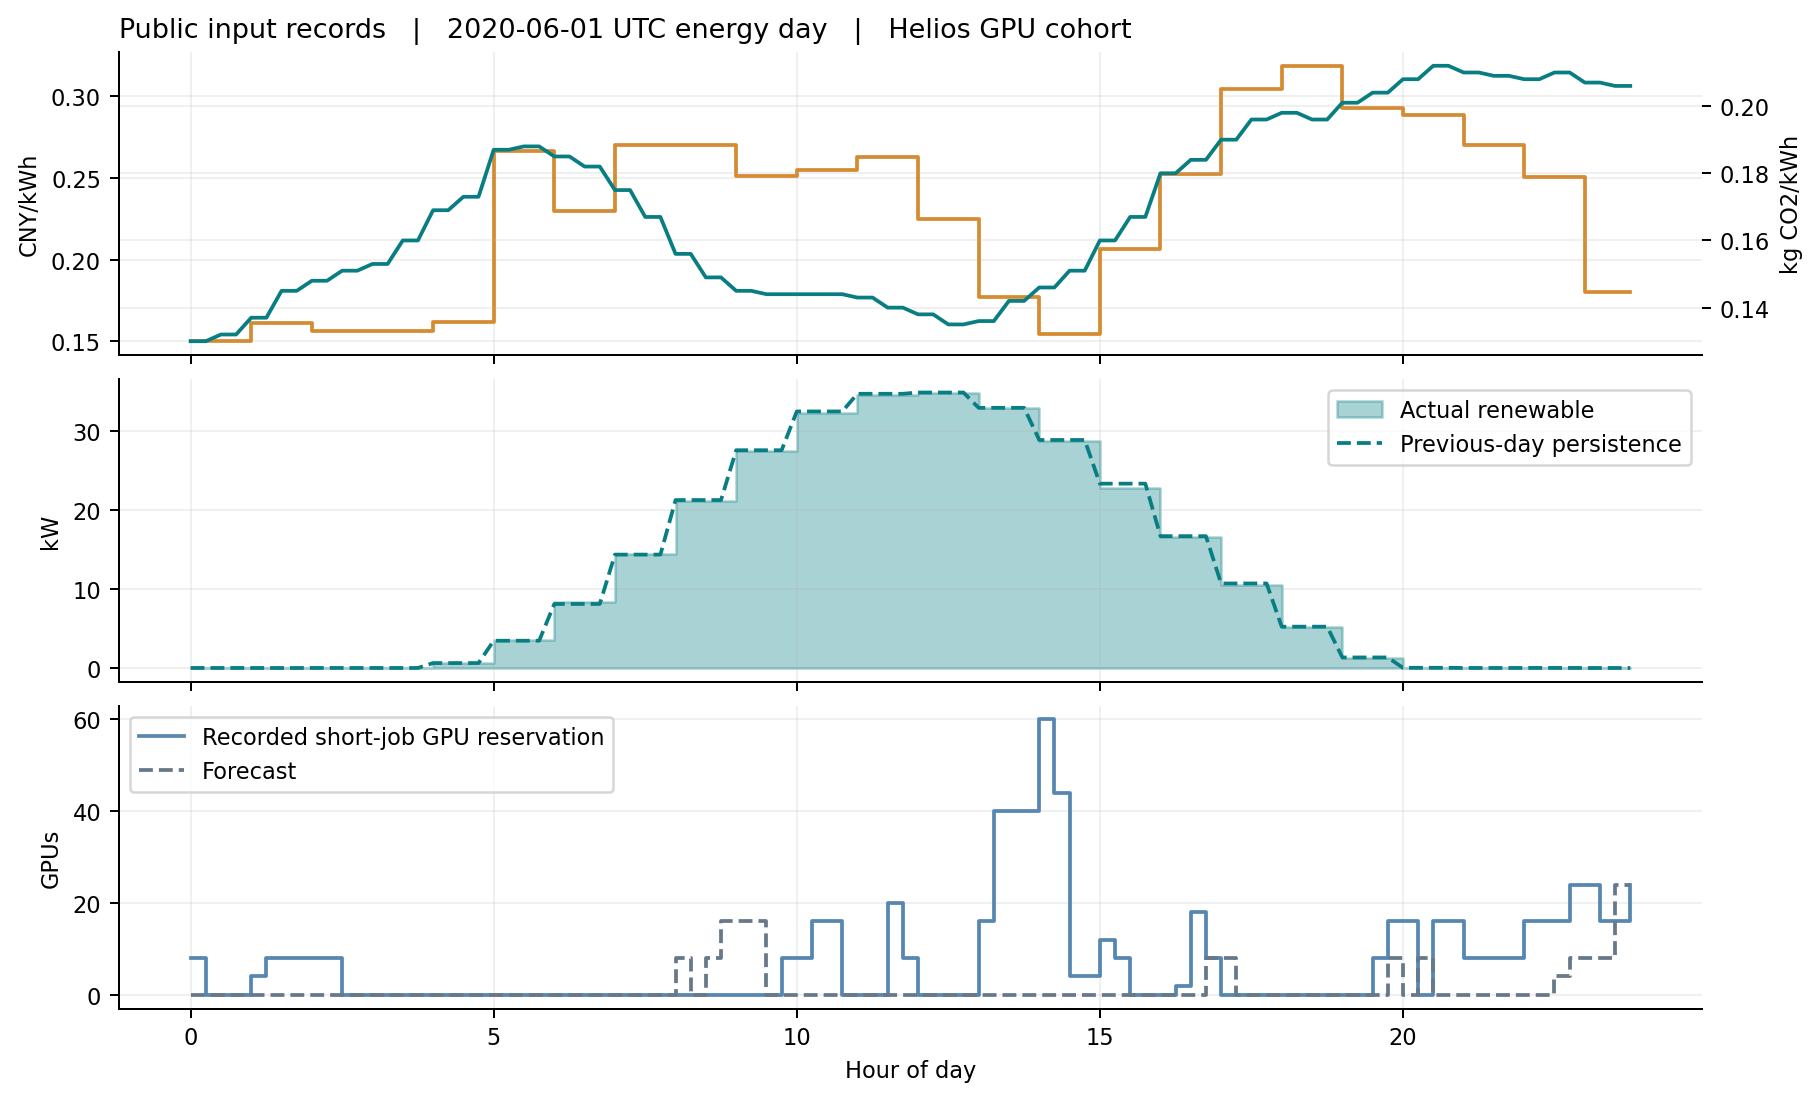
\includegraphics[width=\linewidth,height=260pt,keepaspectratio]{figures/inputs.png}\end{center}
{\small Figure 2. Public signals and derived inputs; solar/background forecasts use previous-day persistence.\par}

\clearpage
\section*{3  Job scheduling and power balance}
\begin{center}\begingroup\setlength{\tabcolsep}{4pt}
\renewcommand{\arraystretch}{1.2}
\fontsize{8.5}{11.90}\selectfont
\begin{tabular}{@{}p{142.60pt}p{332.40pt}@{}}
\toprule
\textbf{Symbol} & \textbf{Meaning and unit} \\
\midrule
t, s; delta t & Slot/start indices; slot duration 0.25 h \\
r, d, L, W; g, p & Release, exclusive deadline, duration, max wait in slots; GPUs, incremental kW \\
z, a; n, N & Binary start and derived activity; background GPUs and capacity \\
G, R, c, u; E & Grid, renewables, battery charge/discharge kW; stored energy kWh \\
kappa, pi, xi & PUE; converted wholesale CNY/kWh; average kg CO2/kWh \\
\bottomrule\end{tabular}\endgroup\end{center}

\begin{equation}
\mathcal F_j=\{s\in\mathbb Z:r_j\le s\le\min(d_j-L_j,r_j+W_j)\},\qquad \sum_{s\in\mathcal F_j}z_{js}=1.
\end{equation}
\begin{equation}
a_{jt}=\sum_{\substack{s\in\mathcal F_j\\s\le t<s+L_j}}z_{js},\qquad\sum_jg_ja_{jt}+n_t\le N_t.
\end{equation}
Exactly one start executes each admitted job for L consecutive slots; finishing at d is allowed, executing in slot d is not. The main pool is homogeneous GPU equivalents. Host memory/CPU and fabric placement remain outside this aggregate model.

\begin{equation}
\sum_{s\in\mathcal F_k}s z_{ks}\ge\sum_{s\in\mathcal F_j}(s+L_j)z_{js},\qquad(j,k)\in\mathcal E_{\rm dep}.
\end{equation}
Parent completion precedes child start when a DAG is supplied. This capability is tested; the public cohort has no supplied edges.

\begin{equation}
P_t^{\rm IT}=P_{\rm base}+q_{\rm inf}n_t+\sum_jp_ja_{jt},\qquad P_t^{\rm fac}=\kappa_tP_t^{\rm IT}.
\end{equation}
\begin{equation}
G_t+R_t+\sum_bu_{bt}=P_t^{\rm fac}+\sum_bc_{bt}.
\end{equation}
\begin{equation}
\begin{aligned}0\le G_t\le\bar G_t,\quad 0\le R_t\le\bar R_t,\quad P_t^{\rm fac}\le\bar P^{\rm fac},\\ |G_t-G_{t-1}|\le\Gamma\quad(t\ge1).\end{aligned}
\end{equation}
{\small Base IT power and incremental job/background power are distinct. Renewables may be curtailed; exports are forbidden. Grid ramp applies between successive slot averages, with no previous-day boundary. Legacy inference\_gpus/training\_gpus fields denote background/scheduled occupancy, not source workload labels.\par}

\clearpage
\section*{4  Storage, objective and solver}
\begin{equation}
E_{b,t+1}=E_{bt}+\eta_b^c c_{bt}\Delta t-\frac{u_{bt}\Delta t}{\eta_b^d}.
\end{equation}
\begin{equation}
E_b^{\min}+E_b^{\rm res}\le E_{bt}\le E_b^{\max},\qquad E_{b0}=E_{bT}=E_b^{\rm init}.
\end{equation}
\begin{equation}
\begin{aligned}0&\le c_{bt}\le(\bar c_b-P_b^{\rm res})v_{bt},\\0&\le u_{bt}\le(\bar u_b-P_b^{\rm res})(1-v_{bt}),\qquad v_{bt}\in\{0,1\}.\end{aligned}
\end{equation}
\begin{center}\begingroup\setlength{\tabcolsep}{4pt}
\renewcommand{\arraystretch}{1.2}
\fontsize{8.3}{11.62}\selectfont
\begin{tabular}{@{}p{85.53pt}p{133.04pt}p{133.04pt}p{107.39pt}@{}}
\toprule
\textbf{Asset} & \textbf{Initial / limits kWh} & \textbf{Charge/discharge kW} & \textbf{Efficiencies} \\
\midrule
LFP & 20 / 4-36 & 10 / 10 & 0.96 / 0.96 \\
Sodium-ion & 3 / 0.6-5.4 & 6 / 6 & 0.94 / 0.94 \\
\bottomrule\end{tabular}\endgroup\end{center}

Sodium-ion retains an extra 1.2 kWh and 2 kW in each direction. Both batteries restore initial energy. Per-battery exclusive modes permit different layers to operate in opposing directions; throughput wear penalizes cycling but does not forbid it under negative prices.

\begin{equation}
C=\Delta t\sum_t(\pi_tG_t+\pi_RR_t)+\lambda Q+\Delta t\sum_{b,t}k_b(c_{bt}+u_{bt}),\quad Q\ge G_t.
\end{equation}
\begin{equation}
M=\Delta t\sum_t\xi_tG_t,\qquad \min C\quad\text{subject to}\quad M\le0.97M_{\rm FIFO}.
\end{equation}
C includes energy, renewable variable cost, a daily peak proxy and AC-throughput wear (LFP 0.035; sodium-ion 0.055 CNY/kWh). M uses average grid-intensity estimates. Charging is counted at import; discharge gets no extra carbon credit. Modeled renewable operational intensity is zero; lifecycle emissions and battery capex are excluded.

HiGHS uses mixed-integer branch-and-bound/cut methods through SciPy milp. Status 0 means requested tolerance reached, 1 a time/resource limit, 2 infeasibility. An LP relaxation supplies a lower bound but fractional jobs are not executable. Stricter-budget incumbents may improve looser problems; lower bounds remain target-specific.

\begin{equation}
L\le C^*\le U,\qquad\operatorname{gap}=\frac{U-L}{|U|}.
\end{equation}
{\small Green U = CNY 205.535943792, L = CNY 205.535831654, gap = 0.000055\%. The model has 1404 variables, 633 binaries and 1082 constraints. The independent audit reconstructs physical/accounting outcomes without reading the MILP matrix.\par}

\clearpage
\section*{5  Dispatch and mechanism comparisons}
\begin{center}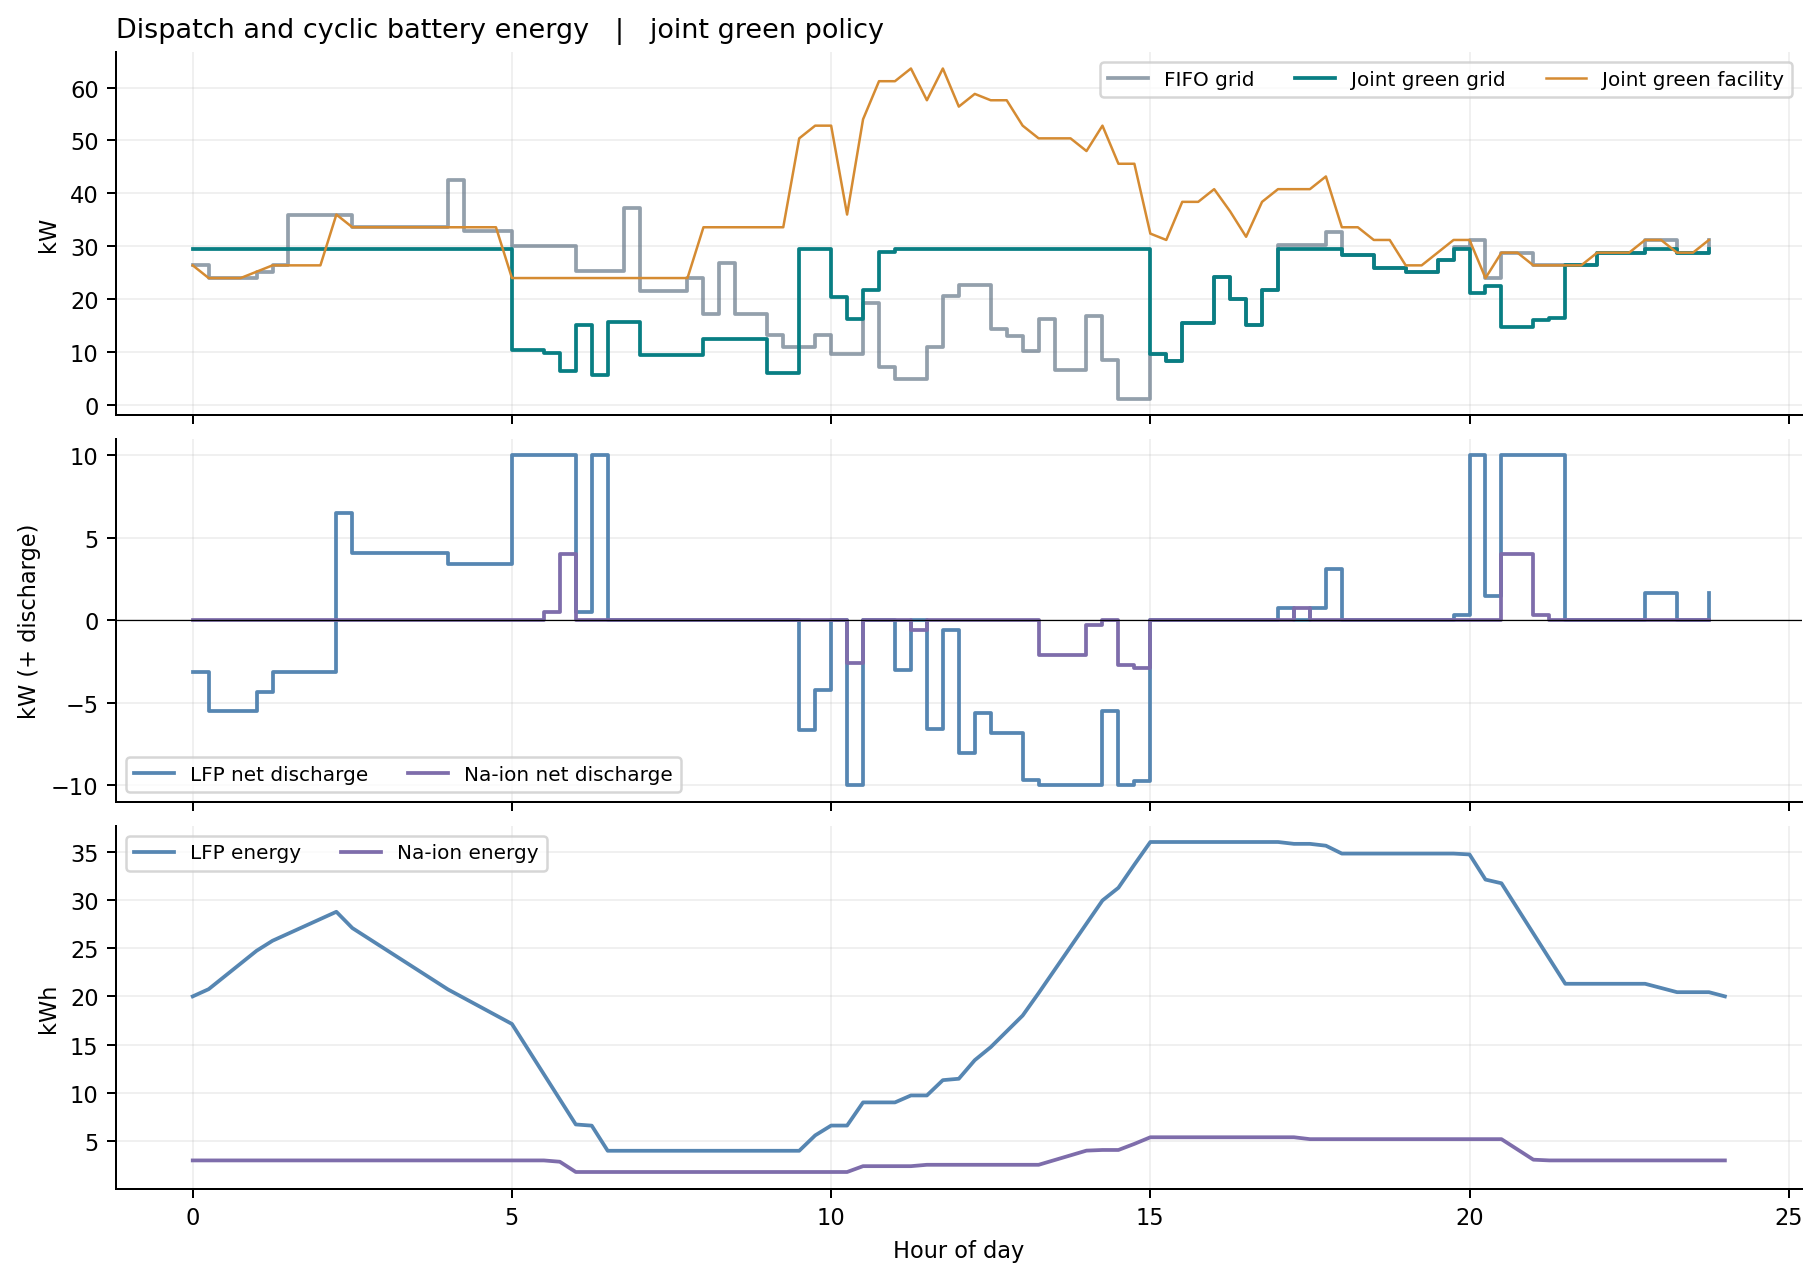
\includegraphics[width=\linewidth,height=310pt,keepaspectratio]{figures/dispatch.png}\end{center}
{\small Figure 3. Recommended dispatch, battery net powers and all 97 energy states.\par}

Facility demand is 855.60 kWh; grid import 563.46 kWh; renewable use 295.91 kWh. Conversion losses add 3.78 kWh. Cyclic terminal energy prevents apparent savings from emptying the initial stock.

\begin{center}\begingroup\setlength{\tabcolsep}{4pt}
\renewcommand{\arraystretch}{1.2}
\fontsize{8.4}{11.76}\selectfont
\begin{tabular}{@{}p{275.56pt}p{91.85pt}p{99.59pt}@{}}
\toprule
\textbf{Same 3\% carbon policy} & \textbf{Cost CNY} & \textbf{Gap / status} \\
\midrule
FIFO + storage & Infeasible & Status 2 \\
Compute only & Infeasible & Status 2 \\
Joint, LFP only & 206.47 & 0.092608\% \\
Joint, both layers & 205.54 & 0.000055\% \\
\bottomrule\end{tabular}\endgroup\end{center}

Cost-only joint scheduling costs CNY 198.08; the selected green requirement adds CNY 7.45. Compute/storage benefits cannot be added as independent savings because each changes the other's operating opportunities.

The LFP-only comparison isolates the second layer's modeled economic increment, not fast-response capability or investment return. Sampled cost/carbon budgets expose trade-offs but do not establish a complete exact frontier. Job CSVs and the offline explorer retain every source-ID schedule.

\clearpage
\section*{6  Public dates and constructed stresses}
\begin{center}\begingroup\setlength{\tabcolsep}{4pt}
\renewcommand{\arraystretch}{1.2}
\fontsize{8.4}{11.76}\selectfont
\begin{tabular}{@{}p{128.29pt}p{109.29pt}p{114.04pt}p{107.39pt}@{}}
\toprule
\textbf{Public date} & \textbf{FIFO service} & \textbf{Green policy} & \textbf{Cost saved} \\
\midrule
2020-06-02 & Feasible & Feasible & 17.28\% \\
2020-06-03 & Feasible & Infeasible & N/A \\
2020-06-04 & Feasible & Feasible & 0.52\% \\
2020-06-05 & Feasible & Feasible & 13.02\% \\
2020-06-08 & Feasible & Infeasible & N/A \\
\bottomrule\end{tabular}\endgroup\end{center}

June 3 and June 8 have feasible cost-only service, but valid minimum-carbon lower bounds exclude the extra 3\% target. The same fixed selection rule applies to all dates. These related observations do not form a facility-wide statistical guarantee.

\begin{center}\begingroup\setlength{\tabcolsep}{4pt}
\renewcommand{\arraystretch}{1.2}
\fontsize{8.4}{11.76}\selectfont
\begin{tabular}{@{}p{213.82pt}p{66.52pt}p{71.27pt}p{107.39pt}@{}}
\toprule
\textbf{Constructed scenario} & \textbf{FIFO} & \textbf{Green} & \textbf{Cost saved} \\
\midrule
cloudy & Yes & Yes & -6.75\% \\
no renewables & Yes & No & N/A \\
flat price & Yes & Yes & 9.87\% \\
price carbon conflict & Yes & Yes & 13.47\% \\
hot day & Yes & Yes & 8.30\% \\
Background GPU surge & Yes & No & N/A \\
grid derating & Yes & Yes & 10.94\% \\
zero flexibility & Yes & No & N/A \\
storage expensive & Yes & Yes & -2.34\% \\
no demand charge & Yes & Yes & 5.22\% \\
high workload & Yes & Yes & 12.63\% \\
impossible grid & No & No & N/A \\
\bottomrule\end{tabular}\endgroup\end{center}

These are perturbations, not historical incidents: cloudy retains 35\% solar; background surge adds 48 GPUs; grid derating halves its cap; hot day sets PUE 1.40. Other cases vary waiting, prices, charges, wear and workload. Negative savings and infeasible targets are retained.

Impossible grid sets both grid and renewable supply to zero. Cyclic batteries cannot create net daily energy; a positive supply-deficit diagnostic proves failure. Passing this necessary energy condition alone does not prove time/resource feasibility. N/A denotes no feasible same-scenario saving comparison.

{\small Independent minimum-carbon runs also separate unattainable environmental targets from workload failures in constructed cases. All five public dates and twelve stresses remain in results/main/.\par}

\clearpage
\section*{7  Online replay, validation and references}
\begin{center}\begingroup\setlength{\tabcolsep}{4pt}
\renewcommand{\arraystretch}{1.2}
\fontsize{8.3}{11.62}\selectfont
\begin{tabular}{@{}p{199.57pt}p{85.53pt}p{85.53pt}p{88.38pt}@{}}
\toprule
\textbf{Online policy} & \textbf{Cost CNY} & \textbf{Carbon kg} & \textbf{Peak kW} \\
\midrule
Default reserve 4 & 228.41 & 98.27 & 41.20 \\
Selected reserve 0 & 226.94 & 98.11 & 40.64 \\
\bottomrule\end{tabular}\endgroup\end{center}

Both replays complete 96 decisions. Past actions/launched starts are locked and future releases hidden. Future solar/background use previous-day persistence; current-slot aggregates are optimistically assumed known at the boundary. Archived carbon forecasts have unknown vintage and do not affect this cost-only policy.

Reserve 0 is selected from 0/2/4/8 on June 2-3 by failures then cost; June 4-5 are separate evaluation. Both default and selected margins survive the declared shock (solar 15\% in slots 40-55, +48 reserved GPUs in 44-51). Neither replay guarantees the offline carbon cap or a global online optimum.

Validation passes 61 unit tests and 55 numerical audits. Sixty brute-force random instances are subcases of three tests. Public-source checks, tampered-result rejection, CLI exits, six-policy desktop/mobile checks and rendered-PDF QA are recorded separately.

{\small Reproduce from README.md and docs/reproduction.md. Run tools/verify\_results.py, rebuild artifacts/report, run browser/PDF QA, refresh tools/build\_docs.py and prepare tools/prepare\_push.py. The curated snapshot verifies copies and reruns numerical/CLI checks. AI assistance: OpenAI Codex supported research, code, experiments and writing; entrants retain responsibility for understanding and truthful contributions.\par}

{\small Limits: assumed deadlines/power/storage, homogeneous GPUs, average carbon and daily peak proxies. No verified request latency, CPU/RAM/topology, transient response, monthly utility bill, TCO/ROI or causal grid-emissions reduction.\par}

\subsection*{References}

{\small \href{https://github.com/S-Lab-System-Group/HeliosData}{[1] HeliosData; Characterization and Prediction of Deep Learning Workloads in Large-Scale GPU Datacenters, SC 2021. CC BY 4.0.}\par}

{\small \href{https://doi.org/10.25832/time_series/2020-10-06}{[2] Open Power System Data, Time series 2020-10-06. Primary ENTSO-E records; source-specific terms retained.}\par}

{\small \href{https://carbonintensity.org.uk/}{[3] UK Carbon Intensity API. National estimates and archived forecasts. CC BY 4.0.}\par}

{\small \href{https://docs.scipy.org/doc/scipy/reference/generated/scipy.optimize.milp.html}{[4] SciPy milp: HiGHS interface, statuses and certificates.}\par}

{\small \href{https://arxiv.org/abs/2106.11750}{[5] Radovanovic et al. 2021. Carbon-Aware Computing for Datacenters.}\par}

{\small \href{https://www.hithium.com/newsroom/latest/details/86.html}{[6] HiTHIUM storage announcement. Motivation; modeled asset ratings remain assumptions.}\par}

{\small [7] Supplied HackSHSID Track 2 statement, project brief and technical specification. [8] IMMC 2025 Problem E, When Watts Meet Bits. Source identities/hashes: data/source\_documents.json. Public-data URLs/hashes/terms: data/raw/manifest.json.\par}


\end{document}
